\section{Differences between participants}

\begin{itemize}
\item {
    \textbf{
        The authors used multiple Fisher's exact tests to examine whether
        there was an effect of sex on any of the dependent variables (independently from each other). A Fisher's exact test is typically
        used to examine association between two categorical variables,
        when both variables only have two options. This is not the case,
        since the responses are on $7$-point scales, and have natural order.
        Give an example of what way the authors could have created categorical data from the response data. There are multiple valid
        answers here. Pick the one you think the reviewers of the article
        would complain the least about, and explain why it is valid for the
        particular Body Ownership question.
    }

    They could have used a binary variable with did/did not experience body ownership.
    Values from $-3$ to $0$ (inclusive) would be "did not experience body ownership" whereas $1$ to $3$ (inclusive) would be "did experience body ownership". This works because negative values disagree with the question of feeling that their virtual hands were their own, and answering $0$ is neutral. These values all represent not feeling body ownership, whereas positive values do.
}

\item {
    \textbf{
        Again taking the body ownership data as an example, describe a
        statistical test that you think is better suited to examine the effect
        of sex (just Male \& Female), regardless of hand representation.
        Use the links provided in the lecture slides to choose a test, and
        if you are not sure, google extra information about possible tests
        (as this is probably how you will approach this problem in the
        future). State the null and alternative hypotheses, and for the
        latter, explicitly state whether it is one-sided or two-sided. List the
        variables and corresponding levels, and all parameters you need
        in your test. Be as specific as possible. You do not need to actually
        perform this test in R.
    }

    A null hypothesis would be "Sex has no effect on perceived Body Ownership", or $H_0 = M_m - M_f = 0$. An alternative hypothesis would be "Sex has an effect on perceived Body Ownership", or $H_a = M_m - M_f \neq 0$.

    The alternative hypothesis is two-sided because it tests whether perceived Body Ownership differs between male and female participants, without predicting which group will report higher scores.

    Body Ownership ($-3$ to $3$) can be considered a dependent variable while participants' sex (Male, Female) is an independent variable.
    Parameters for the test would be sample size and significance level.
}

\item {
    \textbf{
        Using the data set you created in Part II as a starting point (that is,
        where each condition only has a single response value rather than
        three repetitions), visualize the posited correlation between amount
        of VR experience and body ownership responses for each hand
        representation, i.e. choose a visualization, and create one plot for
        each condition. By posited I mean that you do not actually have to
        calculate the correlation or draw a correlation function (see next
        question), just find a way to visualize the data in such way that
        would indicate to readers they should admit or rule out a possible
        correlation. Choose what you think is the best visualization based
        on the type of data we are using, the variables we are investigating, and the problem we are trying to investigate. You will have
        to make decisions here, since there is no perfect answer. Make
        sure your figures contain all the information a reader of a paper
        would need to understand it. Feel free to experiment with plotting
        functions from other R packages than the default packages.
    }

    To create the following graphs we used the ggplot2 package in R.

    \begin{figure}
        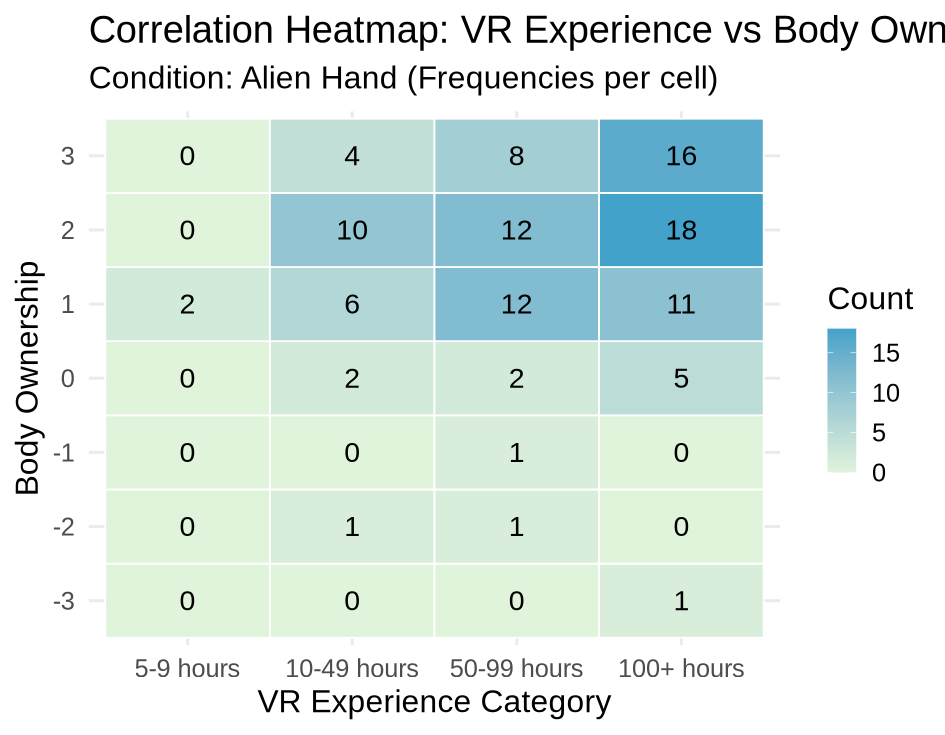
\includegraphics[width=9cm]{alien.png}
        \caption{Body Ownership vs. VR Experience in the alien hand condition.}
        \label{fig:alien}
    \end{figure}

    \begin{figure}
        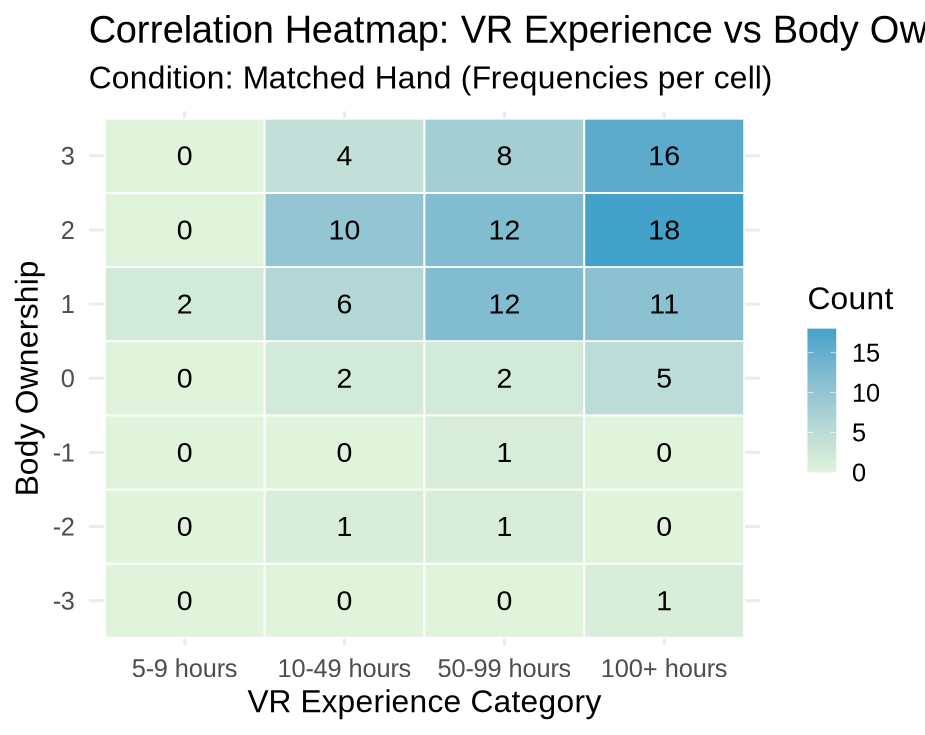
\includegraphics[width=9cm]{matched.png}
        \caption{Body Ownership vs. VR Experience in the matched hand condition.}
        \label{fig:matched}
    \end{figure}

    \begin{figure}
        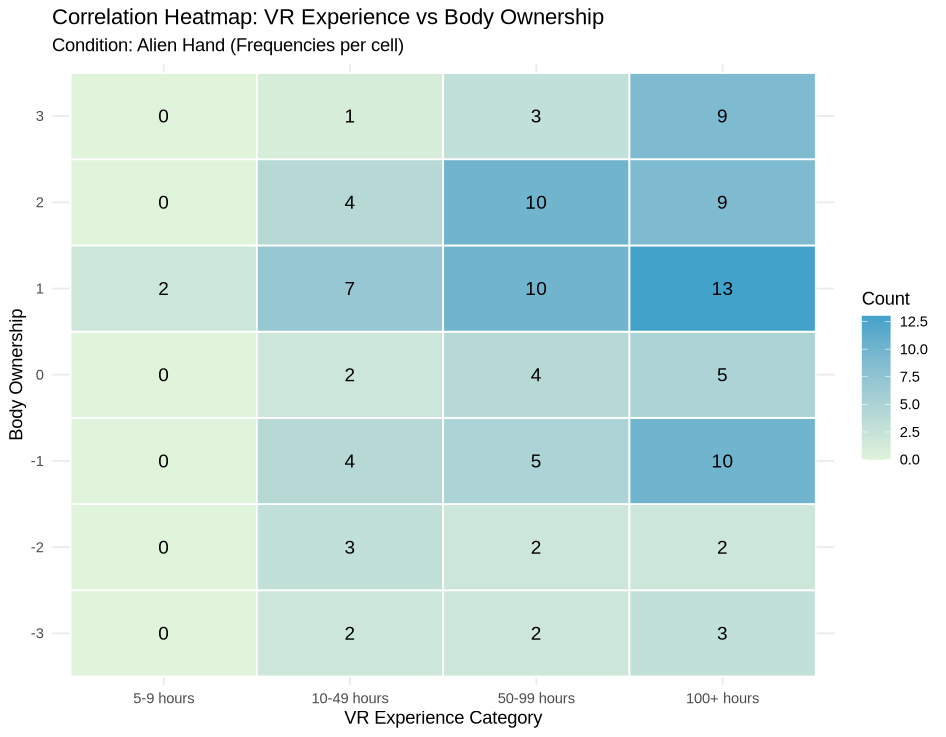
\includegraphics[width=9cm]{mismatched.png}
        \caption{Body Ownership vs. VR Experience in the mismatched hand condition.}
        \label{fig:mismatched}
    \end{figure}
}

\item {
    \textbf{
        Test post-hoc whether there is a positive correlation between VR
        experience and body ownership responses for each hand representation separately, meaning you will have to do multiple comparisons. Choose the correct correlation test using the links in the
        slides and by googling if necessary. Report all relevant results and
        draw a conclusion from your results. If you do not understand
        how to interpret the results in order to give a conclusion, google
        how to interpret the values of your chosen correlation test. You do
        not need to calculate power.
    }

	R input:
    \begin{verbatim}
		
	new_data <- aggregate(Response ~ PID + Condition,
			      data = subset(Responses, Measure == "Body Ownership"),
			      FUN = median)

	combined_data <- merge(new_data, Demographics[, c("PID", "VR Experience")], by = "PID")
	matched_data <- subset(combined_data, Condition == "Matched Hand")
	mismatched_data <- subset(combined_data, Condition == "Mismatched Hand")
	alien_data <- subset(combined_data, Condition == "Alien Hand")


	vr_exp_matched <- as.numeric(factor(matched_data$`VR Experience`, levels = c("5-9 hours", "10-49 hours", "50-99 hours", "100+ hours")))
	vr_exp_mismatched <- as.numeric(factor(mismatched_data$`VR Experience`, levels = c("5-9 hours", "10-49 hours", "50-99 hours", "100+ hours")))
	vr_exp_alien <- as.numeric(factor(alien_data$`VR Experience`, levels = c("5-9 hours", "10-49 hours", "50-99 hours", "100+ hours")))


	spearman_match <- cor.test(matched_data$`Response`, vr_exp_matched ,method = "spearman", exact = FALSE)
	spearman_mismatch <- cor.test(mismatched_data$`Response`, vr_exp_mismatched ,method = "spearman", exact = FALSE)
	spearman_alien <- cor.test(alien_data$`Response`, vr_exp_alien ,method = "spearman", exact = FALSE)

	print(spearman_match)
	print(spearman_mismatch)
	print(spearman_alien)

	    \end{verbatim}

	    R output:
	    \begin{verbatim}
		Spearman's rank correlation rho

	data:  matched_data$Response and vr_exp_matched
	S = 203018, p-value = 0.1624
	alternative hypothesis: true rho is not equal to 0
	sample estimates:
	      rho 
	0.1329072 


	Spearman's rank correlation rho

data:  mismatched_data$Response and vr_exp_mismatched
S = 210259, p-value = 0.2847
alternative hypothesis: true rho is not equal to 0
sample estimates:
      rho 
0.1019782 


	Spearman's rank correlation rho

data:  alien_data$Response and vr_exp_alien
S = 276760, p-value = 0.05472
alternative hypothesis: true rho is not equal to 0
sample estimates:
       rho 
-0.1820486 
    \end{verbatim}
    
    For the Body Ownership to VR Experience correlation in the matched hand condition, the analysis revealed a weak positive correlation that was not statistically significant, $r_s = .13$, $p = .162$.

Similarly, for the mismatched hand condition, a weak positive correlation was observed, which also failed to reach statistical significance, $r_s = .10$, $p = .285$.

In contrast, the alien hand condition demonstrated a weak negative correlation, $r_s = -.18$, $p = .055$. Although this relationship is not statistically significant at the conventional $\alpha = .05$ threshold, it can be considered marginally significant as it closely approaches the cutoff value.}
\end{itemize}
